\documentclass[border=3pt]{standalone}
% Shared TikZ styles for the Ch. 3–8 diagrams (standalone PDFs); extends the Ch. 1 palette (s1_vs_llm_common.tex).
\usepackage[T1]{fontenc}
\usepackage{lmodern}
\usepackage[english]{babel}
\usepackage{amsmath,amssymb}
\usepackage{tikz}
\usetikzlibrary{shapes.geometric,shapes.misc,positioning,fit,arrows.meta,calc,backgrounds,decorations.pathreplacing,patterns}
\definecolor{ioFill}{HTML}{F1F0EC}\definecolor{ioLine}{HTML}{52514E}
\definecolor{modFill}{HTML}{E8F1FB}\definecolor{modLine}{HTML}{2A78D6}
\definecolor{decFill}{HTML}{ECE9F7}\definecolor{decLine}{HTML}{4A3AA7}
\definecolor{postFill}{HTML}{FFF6E0}\definecolor{postLine}{HTML}{EDA100}
\definecolor{okFill}{HTML}{EAF7F1}\definecolor{okLine}{HTML}{1BAF7A}
\definecolor{badFill}{HTML}{FDECEC}\definecolor{badLine}{HTML}{E34948}
\definecolor{nmFill}{HTML}{EFEAF8}\definecolor{nmLine}{HTML}{4A3AA7}
\definecolor{loopRed}{HTML}{E34948}\definecolor{clusterLine}{HTML}{9A9890}\definecolor{ink2}{HTML}{52514E}
\definecolor{orangeA}{HTML}{EB6834}
\tikzset{
  every node/.style={font=\small, align=center},
  io/.style={trapezium, trapezium left angle=72, trapezium right angle=108, trapezium stretches body,
             draw=ioLine, fill=ioFill, thick, inner sep=3pt, minimum height=2.4em},
  model/.style={rectangle, draw=modLine, fill=modFill, very thick, inner sep=4pt, minimum height=2.4em, text width=#1},
  model/.default=3.6cm,
  post/.style={rectangle, draw=postLine, fill=postFill, very thick, inner sep=4pt, minimum height=2.2em, text width=#1},
  post/.default=3.6cm,
  data/.style={cylinder, shape border rotate=90, aspect=0.18, draw=okLine, fill=okFill, very thick, inner sep=3pt, minimum height=2.6em, text width=#1},
  data/.default=2.4cm,
  decision/.style={diamond, aspect=2.1, draw=decLine, fill=decFill, very thick, inner sep=1pt},
  outcome/.style={rounded rectangle, draw=#1, thick, inner sep=4pt, minimum height=2em},
  arrow/.style={-{Latex[length=2mm]}, thick, ioLine},
  dashedarrow/.style={-{Latex[length=2mm]}, thick, ioLine, dashed},
  loop/.style={-{Latex[length=2.4mm]}, line width=1.4pt, loopRed},
  cluster/.style={draw=clusterLine, dashed, rounded corners=3pt, inner sep=7pt},
  clusterlabel/.style={font=\small\bfseries, text=ioLine},
  note/.style={font=\footnotesize, text=ink2},
  tok/.style={rectangle, draw=ioLine, fill=ioFill, thin, inner sep=2pt, minimum height=1.6em, font=\footnotesize},
  vmark/.style={rectangle, draw=orangeA, fill=postFill, thick, inner sep=2pt, minimum height=1.6em, font=\footnotesize\ttfamily},
}

\begin{document}\hyphenpenalty=10000\exhyphenpenalty=10000
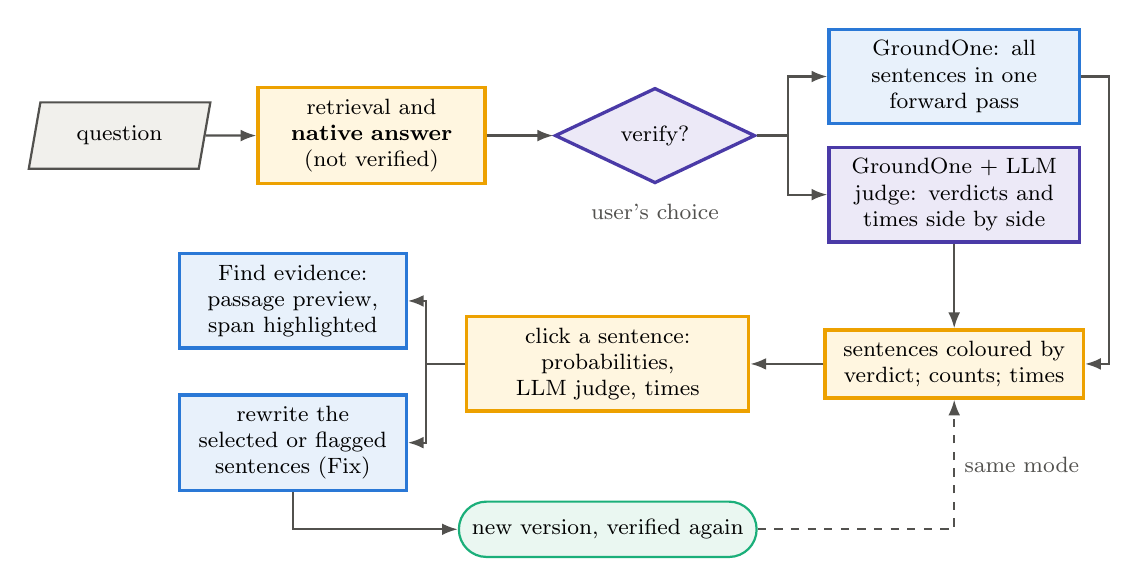
\begin{tikzpicture}
  \node[io, text width=1.8cm, font=\footnotesize] (q) at (0,0) {question};
  \node[post=2.6cm, font=\footnotesize] (a) at (3.2,0) {retrieval and\\\textbf{native answer}\\(not verified)};
  \node[decision, font=\footnotesize, text width=1.8cm] (v) at (6.8,0) {verify?};
  \node[model=2.9cm, font=\footnotesize] (g1) at (10.6,0.75) {GroundOne: all sentences in one forward pass};
  \node[model=2.9cm, font=\footnotesize, draw=decLine, fill=decFill] (gj) at (10.6,-0.75) {GroundOne + LLM judge: verdicts and times side by side};
  \node[post=3.0cm, font=\footnotesize] (col) at (10.6,-2.9) {sentences coloured by verdict; counts; times};
  \node[post=3.3cm, font=\footnotesize] (sel) at (6.2,-2.9) {click a sentence:\\probabilities, LLM judge, times};
  \node[model=2.6cm, font=\footnotesize] (ev) at (2.2,-2.1) {Find evidence: passage preview, span highlighted};
  \node[model=2.6cm, font=\footnotesize] (rw) at (2.2,-3.9) {rewrite the selected or flagged sentences (Fix)};
  \node[outcome=okLine, fill=okFill, font=\footnotesize] (nv) at (6.2,-5.0) {new version, verified again};
  \draw[arrow] (q) -- (a);
  \draw[arrow] (a) -- (v);
  \draw[arrow] (v.east) -- ++(0.4,0) |- (g1.west);
  \draw[arrow] (v.east) -- ++(0.4,0) |- (gj.west);
  \draw[arrow] (gj) -- (col);
  \draw[arrow] (g1.east) -- ++(0.35,0) |- (col.east);
  \draw[arrow] (col) -- (sel);
  \draw[arrow] (sel.west) -- ++(-0.5,0) |- (ev.east);
  \draw[arrow] (sel.west) -- ++(-0.5,0) |- (rw.east);
  \draw[arrow] (rw.south) |- (nv.west);
  \draw[dashedarrow] (nv.east) -| node[right, note, pos=0.75] {same mode} (col.south);
  \node[note, anchor=north] at (6.8,-0.75) {user's choice};
\end{tikzpicture}
\end{document}
